\chapter{Random Variables and Probability Distributions} \label{ch:rv}

The definition of random variable has been introduced in earlier chapter. This chapter digs deeper into the different types and properties of random variables, and how we describe a random variable.

\section{Discrete and Continuous Random Variables}

A random variable may be discrete or continuous depending on the sample space of the variable.

\subsection{Discrete Random Variables}

If a random variable $X$ takes only discrete values $x_1, x_2, ...$, it is called a discrete random variable.
The probability of $X$ taking a particular value $x$ is denoted by $P(X=x)$. Sometimes for simplicity, it is simply denoted by function $f(x)=P(X=x)$ when there is no ambiguities. In this case, $P(X=x)$ and $f(x)$ are called the \textit{probability function} (also known as \textit{probability mass function}) of $X$.

Furthermore, define $P(X\leq x)$ or $F(x)$ as the \textit{cumulative distribution function}. It is easy to prove that $F(x)$ is nondecreasing, and $\lim_{x\rightarrow 0}F(x)=0$, $\lim_{x\rightarrow \infty}F(x)=1$. Also, $F(x)$ ``jumps'' at each $P(X=x_k)>0$ and it is continuous from the right.

\subsection{Continuous Random Variables}

A random variable $X$ may also take continuous values in many applications. For example, let $X$ denote the time consumption to finish a task, which can be any value above $0$ hours.

In this case, the chance for $X$ to take a precise value, say for the student to finish his homework using precisely 25 minutes 13 seconds and 750 milliseconds, is very small (in fact, mathematically zero). The probability function $P(X=x)$ becomes useless. The cumulative distribution function $F(x) = P(X\leq x)$ still makes sense, as it essentially calculates the probability of $X$ given by not a precise value but within a range.

Inspired by this, define \textit{probability density function (PDF)} or $f(x)$ for continuous random variable as follows. The probability density function $f(x)$ is such that
\begin{eqnarray}
  P(a < X < b) &=& \int_{a}^{b}f(x)dx \nonumber
\end{eqnarray}
Therefore,
\begin{eqnarray}
  F(x) &=& P(X\leq x) \nonumber \\
  &=& \int_{-\infty}^{x} f(\epsilon)d\epsilon \nonumber
\end{eqnarray}
Notice that $f(x)$ itself is not probability. It is $f(x)dx$ accumulating in range $x \in (a, b)$ that forms the probability, hence the name ``probability density''.

In science and engineering problems, continuous random variables are more common than discrete random variables. Therefore, the main focus of this notebook from this point on would be continuous signals. Discrete random variables can sometimes be taken as a special case of continuous random variables with impulse PDF.

\section{Joint Distribution}

Joint distribution is used to study the correlation of multiple random variables. It is widely used in system identification where insights of unknown variables are obtained by observing the known variables, assuming their correlation is known.

\subsection{Joint Probability Density Function}

Consider two random variables $X$ and $Y$. In the case of discrete variables, define joint probability function and joint cumulative distribution function as follows.
\begin{eqnarray}
  f(x, y) &=& P\left(X=x, Y=y\right) \nonumber \\
  F(x, y) &=& P\left(X\leq x, Y\leq y\right) \nonumber \\
  &=& \sum_{u\leq x}\sum_{v\leq y}f(u, v) \nonumber
\end{eqnarray}

In the case of continuous random variables, joint PDF of $X$ and $Y$ is such that
\begin{eqnarray}
  \int_{x=a}^{b}\int_{y=c}^{d} f(x, y) dxdy &=& P\left(a < X < b, c < y < d \right) \label{eq:jointpdf}
\end{eqnarray}
Integrate \eqref{eq:jointpdf} w.r.t an axis gives the PDF of the other variable. For example,
\begin{eqnarray}
  \int_{y=-\infty}^{\infty} f(x, y) &=& f_X(x) \label{eq:jointpdfdowngrade}
\end{eqnarray}
which becomes a function of a single variable, $x$. Here $f_X(x)$ is nothing but the PDF of $X$, completely ignoring the other variable $Y$.

We can define cumulative distribution function for joint distribution likewise as follows.
\begin{eqnarray}
  F(x, y) &=& P(X \leq x, Y \leq y) \nonumber \\
  &=& \int_{u=-\infty}^{x}\int_{v=-\infty}^{y}f(u, v)dudv \nonumber \\
  F_X(x) &=& P(X \leq x) \nonumber \\
  &=& \int_{u=-\infty}^{x}\int_{v=-\infty}^{\infty}f(u, v)dudv \nonumber
\end{eqnarray}

\subsection{Conditional Distribution}

As introduced earlier, \eqref{eq:jointpdfdowngrade} gives the PDF of $X$ by completely ignoring $Y$. In other words, it is the best guess of $X$ (in the form of PDF) when there is no measurement of $Y$.

Conditional distribution, on the other hand, try to find the best guess of $X$ when $Y$ is measured. For example, from \eqref{eq:jointpdf}, let $Y$ be measured by a fixed value $y$, and we would like to calculate $f_{X|Y}(x |Y=y)$, i.e., the PDF of $X$ given the known information $Y=y$. In many literatures, $f_{X|Y}(x |Y=y)$ is denoted by $f_{X|Y}(x|y)$ for simplicity.

The conditional PDF $f_{X|Y}(x|y)$ can be obtained as follows. It is essentially Bayes' rule applied on continuous variables.
\begin{eqnarray}
  f_{X|Y}(x|y) &=& \dfrac{f(x, y)}{f_Y(y)} \label{eq:conditionalpdf1}
\end{eqnarray}
Equation \eqref{eq:conditionalpdf1} is given as an analytical equation of both $x$ and $y$. Just substitute the measured value of $y$ into \eqref{eq:conditionalpdf1} to get a function of $x$ alone. Since \eqref{eq:conditionalpdf1} itself is a PDF of $X$, its integration w.r.t $x$ is certainly $1$. This can be easily verified as follows.
\begin{eqnarray}
  \int_{x=-\infty}^{\infty}f_{X|Y}(x|y)dx &=& \int_{x=-\infty}^{\infty}\dfrac{f(x, y)}{f_Y(y)}dx \nonumber \\
  &=& \dfrac{\int_{x=-\infty}^{\infty}f(x, y)dx}{f_Y(y)} \nonumber \\
  &=& \dfrac{f_Y(y)}{f_Y(y)} \nonumber \\
  &=& 1 \nonumber
\end{eqnarray}
for any $y$. Notice that given a particular value of $y$, $f_Y(y)$ is a constant value independent of $x$, hence can be taken out from the integration in the intermediate derivation.

If $X$ and $Y$ are independent variables, $f(x,y) = f_X(x)f_Y(y)$. In this case, \eqref{eq:conditionalpdf1} becomes
\begin{eqnarray}
  f_{X|Y}(x|y) &=& f_X(x) \nonumber
\end{eqnarray}
which implies that the information of $Y=y$ does not affect our understanding of $X$, just as if the information is completely ignored.

\subsection{Parameter Estimation with Conditional Distribution}

Equation \eqref{eq:conditionalpdf1} is widely used in parameter estimation. Let $\theta$ be the parameter(s) to be estimated, and $x$ the measurement(s) that reflects $\theta$ via measurement model $f(\theta, x)$ which is given in the form of joint distribution of $\theta$ and $X$. The model is known as priori knowledge. Notice that parameters and measurements are correlated via joint PDF but not deterministic due to measurement noise and other uncertain factors.

Given measurement(s) $X=x$, the posteriori estimation of $\theta$ (in the form of PDF) can be obtained as follows. From \eqref{eq:conditionalpdf1},
\begin{eqnarray}
  f_{\theta|X}(\theta|x) &=& \dfrac{f_{X|\theta}(x|\theta)f_\theta(\theta)}{f_X(x)} \label{eq:conditionalpdf2}
\end{eqnarray}
where on the right side $f_{X|\theta}(x|\theta)$ is known as the \textit{likelihood function} that describes the likelihood of measuring $X=x$ if the actual parameter(s) is $\theta$, $f_\theta(\theta)$ the \textit{priori} knowledge of the distribution of $\theta$, and finally $f_X(x)$ which is known as \textit{evidence}, in this case a constant known value given $X=x$.

Equation \eqref{eq:conditionalpdf2} can be memorized as follows.
\begin{eqnarray}
  \textup{posteriori} &=& \dfrac{\textup{likelihood}\times\textup{priori}}{\textup{evidence}} \nonumber
\end{eqnarray}

An estimation of $\theta$ can then be obtained by simply calculate its expectation as follows
\begin{eqnarray}
  \textup{E}(\theta) &=& \int_{-\infty}^{\infty} f_{\theta|X}(\theta|x) d\theta \nonumber
\end{eqnarray}

Terms \textit{priori} and \textit{prior}, \textit{posteriori} and \textit{posterior} can be used interchangeably, respectively.

\subsection{Geometric Probability}

Geometric probability is an extension of classical probability to continuous random variables. Similar with classical probability where it is prerequisite that all elementary events share the same probability, in geometric probability it is assumed that all random variables (usually 2 or 3 variables in total) are uncorrelated and uniformly distributed. The probability of an event happening then can be obtained by measuring the area or volume of the event.

Theory wise, geometric probability is just one of the many joint PDF applications that is simple, intuitive and useful. An example is used to illustrate the use of geometric probability.

\begin{shortbox}
\Boxhead{Geometric Probability Example}
Consider two people trying to meet up at the park, but they forgot to tell each other the time to meet. Both of them will arrive at the park at anytime between $8:00$ AM and $9:00$ AM with equal chance, and wait for the other for 15 minutes or until $9:00$ AM, whichever is earlier, and then will leave the park if the other does not show up.

Calculate the chance of the two people successfully meeting up.
\end{shortbox}

Draw the sample space in a 2-D plot as shown in Fig. \ref{fig:geometricprobexp}, where the x-axis and y-axis are the arriving time of the two people, respectively. The shaded area represents the samples where the two would meet up successfully.
\begin{figure}
	\centering
	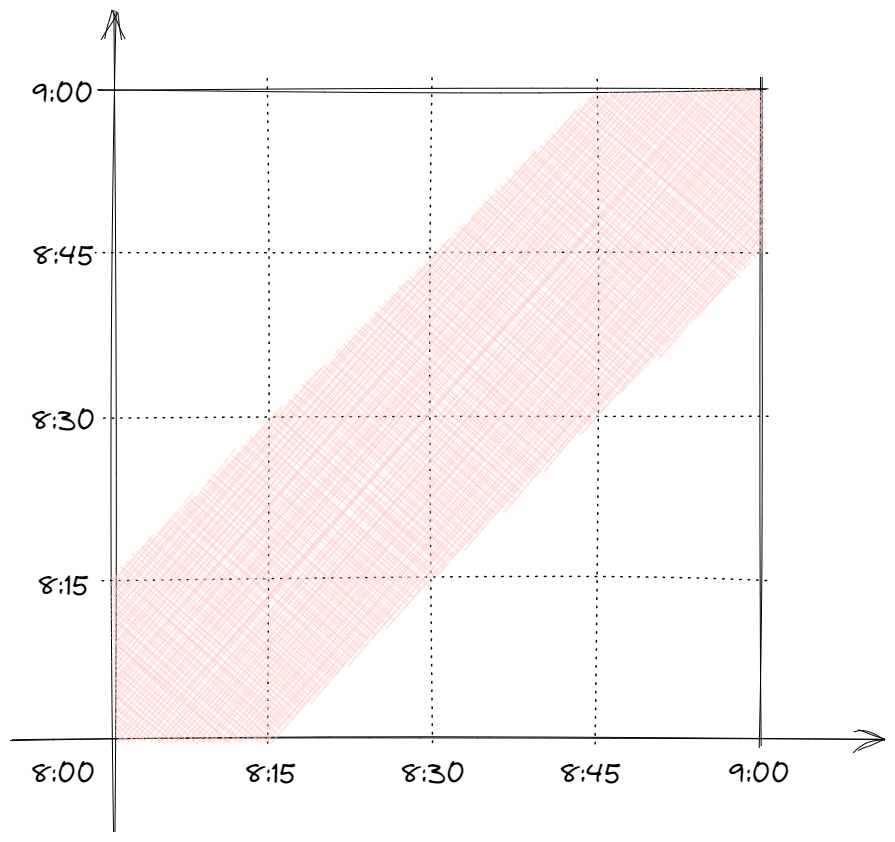
\includegraphics[width=250pt]{chapters/ch-random-variables/figures/geometricprobexp.png}
	\caption{Sample space of two people arriving at part from 8:00 AM to 9:00 AM.} \label{fig:geometricprobexp}
\end{figure}
Divide the shared area by the total sample space area to get $P=7/16=43.75\%$ which is the probability that the two would meet up successfully.

\section{Probability Density Function of Derived Variables}

Let $X$ be a random variable with PDF $f_X(x)$. Let $U$ be another random variable which is a function of $X$ via $U=\phi(X)$. The PDF of $U$ can be calculated as follows. For simplicity, assume that $U=\phi(X)$ is a injective function (one-to-one function), and $X=\phi^{-1}(U)=\psi(U)$. In that case, the PDF of $U$, $g(u)$, can be obtained as follows.
\begin{eqnarray}
  g(u) &=& \left|\psi\textprime(u)\right|f\left(\psi(u)\right) \nonumber
\end{eqnarray}
For example, let $U=aX$, $X=\frac{U}{a}$.
\begin{eqnarray}
  g(u) &=& \dfrac{1}{a}f\left(\dfrac{u}{a}\right) \nonumber
\end{eqnarray}

Let $X$, $Y$ be two random variables with joint distribution $f(x, y)$. Let $U=X+Y$. The PDF of $U$ can be obtained as follows.
\begin{eqnarray}
  g(u) &=& \int_{-\infty}^{\infty} f(x, u-x)dx \label{eq:conditionalpdf3}
\end{eqnarray}
In the special case where $X$ and $Y$ are independent, $f(x, y) = f_X(x)f_Y(y)$, and \eqref{eq:conditionalpdf3} becomes
\begin{eqnarray}
  g(u) &=& \int_{-\infty}^{\infty} f_X(x)f_Y(u-x)dx \nonumber \\
  &=& f_X * f_Y \nonumber
\end{eqnarray}
where $*$ denotes the convolution operator.
